\documentclass{article}

\usepackage{arxiv}

\usepackage[utf8]{inputenc} % allow utf-8 input
\usepackage[T1]{fontenc}    % use 8-bit T1 fonts
\usepackage{hyperref}       % hyperlinks
\usepackage{url}            % simple URL typesetting
\usepackage{booktabs}       % professional-quality tables
\usepackage{amsfonts}       % blackboard math symbols
\usepackage{amsmath}
\usepackage{nicefrac}       % compact symbols for 1/2, etc.
\usepackage{microtype}      % microtypography
\usepackage{graphicx}
\usepackage{natbib}
\usepackage{doi}
\usepackage{csquotes}


\def \thetitle {Wave Arbitrage: A Disproof of the Efficient Market Hypothesis}
\title{\thetitle}

\date{February 15, 2021}

\author{
  \href{https://orcid.org/0000-0001-6450-3262}{
\includegraphics[scale=0.06]{orcid.pdf}\hspace{1mm}Logan P.~Evans}
  \\ \texttt{loganpevans@gmail.com}
}

% Uncomment to override  the `A preprint' in the header
%\renewcommand{\headeright}{Technical Report}
%\renewcommand{\undertitle}{Technical Report}
\renewcommand{\shorttitle}{\textit{arXiv} Template}

%%% Add PDF metadata to help others organize their library
%%% Once the PDF is generated, you can check the metadata with
%%% $ pdfinfo template.pdf
\hypersetup{
pdftitle={\thetitle},
pdfsubject={econ.EM, econ.TH},
pdfauthor={Logan P.~Evans},
pdfkeywords={Efficient Market Hypothesis, Wave Arbitrage},
}

\newtheorem{theorem}{Theorem}
\newtheorem{corollary}{Corollary}
\newtheorem{lemma}{Lemma}

\begin{document}
\maketitle

\begin{abstract}
  Wave arbitrage is a trading strategy that has a higher expected return rate
  than the buy-and-hold strategy when a ``fair game'' dictates price
  fluctuations. This is a contradiction to the efficient market hypothesis. We
  compare the wave arbitrage and buy-and-hold strategies for SP500 stocks from
  late 2016 to early 2021 and demonstrate that wave arbitrage produces excess
  returns, even accounting for trading fees.
\end{abstract}

% keywords can be removed
\keywords{Efficient Market Hypothesis \and Wave Arbitrage}

\section{Introduction}

The efficient market hypothesis has been a useful way to think about markets for
over half a century. According to \citet{fama1970},

\begin{displayquote}
A market in which prices always “fully reflect” all available information is called “efficient.”
\end{displayquote}

There are several tests that can show that a market is inefficient.
\citet{fama1976} summarized one of those tests with the observation, "... in an
efficient market, trading rules with abnormal returns do not exist.” In other
words, if the efficient market hypothesis is true, it is impossible to beat the
buy-and-hold strategy except through luck.

Wave arbitrage is similar to tidal power generators. As ocean waves come in
or go out, the water turns a water wheel and generates electricity. With wave
arbitrage, when the stock price moves up or down, the algorithm harvests some
of the energy of that wave by selling when the price rises and buying when the
price falls. The algorithm guarantees that a trader sells when prices are at a
peak and buys when prices are at their lowest point.

The wave arbitrage strategy will only work if the market fluctuates. However,
fluctuation is a defining attribute of the stock market. New information causes
a market to wobble as traders react to that news, and there will always be more
news. According to \citet{brooks2014}, an acquaintance of J. P. Morgan once
asked him what the market would do, to which Morgan replied, “It will
fluctuate.”

\section{Wave Arbitrage}

Consider a scenario where a trader is fully invested in two companies and at
time $t$ must decide the proportion of their assets invested in each share.

In some situations it is easy to determine whether a trader’s portfolio is on
the correct side of a trade. If the trader is holding only shares of stock $i$
and the price $p_i$ of that stock increases while $p_j$ does not increase, then
the trader is on the correct side of the trade. However, what about situations
where the trader is not fully invested in one stock? We use a geometric mean to
decide whether a portfolio comes out ahead or behind on any individual event.

Let $s_i$ represent the number of shares a portfolio holds of security $i$. The
value of the portfolio, using $s_i$ as the basis of measurement, is
$S_i = s_i + \frac{s_j p_j}{p_i}$. However, since both $S_i$ and $S_j$ are both
reasonable representations for the value of a portfolio, we take the geometric
mean of the two representations and obtain

\begin{equation}
\label{eq:g_def}
  G = \sqrt{ \bigg( s_i + \frac{s_j p_j}{p_i} \bigg)
             \bigg( s_j + \frac{s_i p_i}{p_j} \bigg)
           }
    = \frac{s_i p_i + s_j p_j}{\sqrt{p_i p_j}}.
\end{equation}

Let $\alpha_i$ represent the proportion of the portfolio invested in security
$i$. At time $t$, the prices $p_i$ are constant, so $G$ has the property that
for any $\alpha_i$, $G$ is a constant value. More plainly, if a trader can
ignore exchange fees, then the value of $G$ is the same both before and after
each transaction.

Outside of rebalance events, $G$ is a function of the prices $p_i$ and $p_j$.
To find the minimum, we take the derivative with respect to $p_i$:

\begin{equation}
\begin{aligned}
  G &= \frac{s_i p_i + s_j p_j}{\sqrt{p_i p_j}} \\
  \frac{dG}{dp_i} &= \frac{p_j (s_i p_i - s_j p_j)}{2 (p_i p_j)^{\frac{3}{2}}} \\
\end{aligned}
\end{equation}

Assuming prices are always greater than zero, the only root is at
\begin{equation}
\label{eq:balance}
  s_i p_i = s_j p_j .
\end{equation}

This represents the global minimum. This leads to

\begin{lemma}
\label{lemma}
  The sequence $\{G\}$ will monotonically increase if the only actions performed
  is to rebalance the portfolio so that $\alpha_i = \frac{1}{2}$.
\end{lemma}

This observation is the key to the wave arbitrage algorithm. Fluctuations in the
market will cause the value of $G$ to change, but the value will never be less
than $G_t$, the value of $G$ after rebalancing $\alpha_i = \frac{1}{2}$ at
time $t$. The trigger for rebalance events can be selected so that
$G_{t+1} > G_t$ accounting for any transaction fees.

Since all share quantities and price increments have a minimum size, there is
some smallest amount by which $G$ can change. Thus, not only does $G$ increase
monotonically, it diverges.

If the portfolio is holding cash as one of its two assets, then
\ref{eq:balance} simplifies to $d = s p$. This leads to

\begin{corollary}
  If price $p$ is observed at times $t$ and $t+1$, and if the only
  transactions made to a cash and single share portfolio are to rebalance cash
  and shares to equal ratios, then the value of the portfolio will be strictly
  greater at time $t + 1$ if at least one rebalance event has occurred.
\end{corollary}

\section{Disproof of the Efficient Market Hypothesis}
\label{sec:disproof}

\citet{fama1970} describes a test that can show that a market is
inefficient. Fama described the total excess market value at $t+1$ as

\begin{equation}
  V_{t+1}
    = \sum_{j=1}^n \alpha_j (\Phi_t) [ r_{j,t+1} - E(\tilde{r}_{j,t+1} | \Phi_t)].
\end{equation}

The value $\alpha_j (\Phi_t)$ represents the proportion of assets invested in
security $j$, $r_{j,t+1}$ is the actual return at $t+1$, and
$E(\tilde{r}_{j,t+1} | \phi_t)$ is the expected equilibrium returns given the
available information $\Phi_t$. Using the ``fair game'' property, meaning that price movements follow a martingale, he concludes

\begin{equation}
\label{eq:excess_returns}
  E(\tilde{V}_{t+1} | \Phi_t)
    = \sum_{j=1}^n \alpha_j (\Phi_t) E(\tilde{z}_{j,t+1} | \Phi_t)
    = 0.
\end{equation}

In other words, no strategy will outperform any other strategy. Since the
buy-and-hold strategy avoids all trading costs, it can be used as a benchmark.
If any strategy does have a higher expected value than the buy-and-hold
strategy, the market is inefficient.

While \citet{fama1970} put this forward as a test that can determine if a
market is inefficient, he also provided this warning:

\begin{displayquote}
  But we should note right off that, simple as it is, the assumption that the
  conditions of market equilibrium can be stated in terms of expected returns
  elevates the purely mathematical concept of expected value to a status not
  necessarily implied by the general notion of market efficiency. The expected
  value is just one of many possible summary measures of a distribution of
  returns, and market efficiency per se (i.e., the general notion that prices
  ``fully reflect'' available information) does not imbue it with any special
  importance. Thus, the results of tests based on this assumption depend to
  some extent on its validity as well as on the efficiency of the market. But
  some such assumption is the unavoidable price one must pay to give the theory
  of efficient markets empirical content.
\end{displayquote}

In other words, without tying the efficient market hypothesis to an assumption
about expected value, the hypothesis is little more than a tautology.

Since Lemma \ref{lemma} implies that $\{G\}$ monotonically increases under wave
arbitrage, the goal is to determine whether the expected value of the portfolio
also increases.

Inspecting the expected value of wave arbitrage, we let
$S_i = s_i + \frac{s_j p_j}{p_i}$ represent the potential number of shares of
security $i$ that a portfolio can produce if all shares of security $j$ are sold
and the proceeds are used to buy shares of security $i$. Since \ref{eq:g_def}
is the geometric mean of two quantities, we can use the inequality of
arithmetic and geometric means to write

\begin{equation}
  G = \sqrt{S_i S_j} \leq \frac{S_i + S_j}{2}.
\end{equation}

When using wave arbitrage, since the sequence $\{G\}$ grows monotonically and
diverges due to Lemma \ref{lemma}, the arithmetic mean of $S_i$ and $S_j$ will
also diverge. From this we conclude that the expected number of potential
shares increases:

\begin{equation}
  E(S_{i,t+1}) > E(S_{i,t}).
\end{equation}

Under the buy-and-hold strategy, the number of shares held does not change, but
$S_i$ is a function of the prices and can change. However, the expected returns
from security $i$ is equal to the expected returns from security $j$; if that
were not the case, an investor could allocate all of their assets to one or the
other of the securities and have an abnormally high expected return. This
implies that the expected price change $\delta$ is equal for the two assets.
However, if $E (p_{i,t+1}) = \delta p_{i,t}$ and $E (p_{j,t+1}) = \delta
p_{j,t}$, then

\begin{equation}
  E (S_{i,t+1}) = s_i + \frac{s_j (\delta p_{j,t})}{\delta p_{i,t}} = E (S_{i}).
\end{equation}

Therefore, the expected return rate for wave arbitrage is higher than the
expected return rate for buy-and-hold and Equation \ref{eq:excess_returns} is
false. ``Fair game'' markets are inefficient.

\section{Empirical Observation}

The effect size of wave arbitrage is small but observable. The \citet{IEX}
dataset provides a record of all transactions on the Investors Exchange since
late 2016. Using this dataset, we created a simulation that modeled both the
buy-and-hold and wave arbitrage algorithms. The exchange charges a fee of
\$0.0009 per share traded. The simulation selects two assets and generates a
buy-and-hold portfolio and a wave arbitrage portfolio and then attempts to
rebalance the wave arbitrage portfolio after every transaction in the back
test. The portfolio values at each time $t$ are recorded, and after a period of
one year the return is stored in a histogram.

\begin{figure}[h!]
  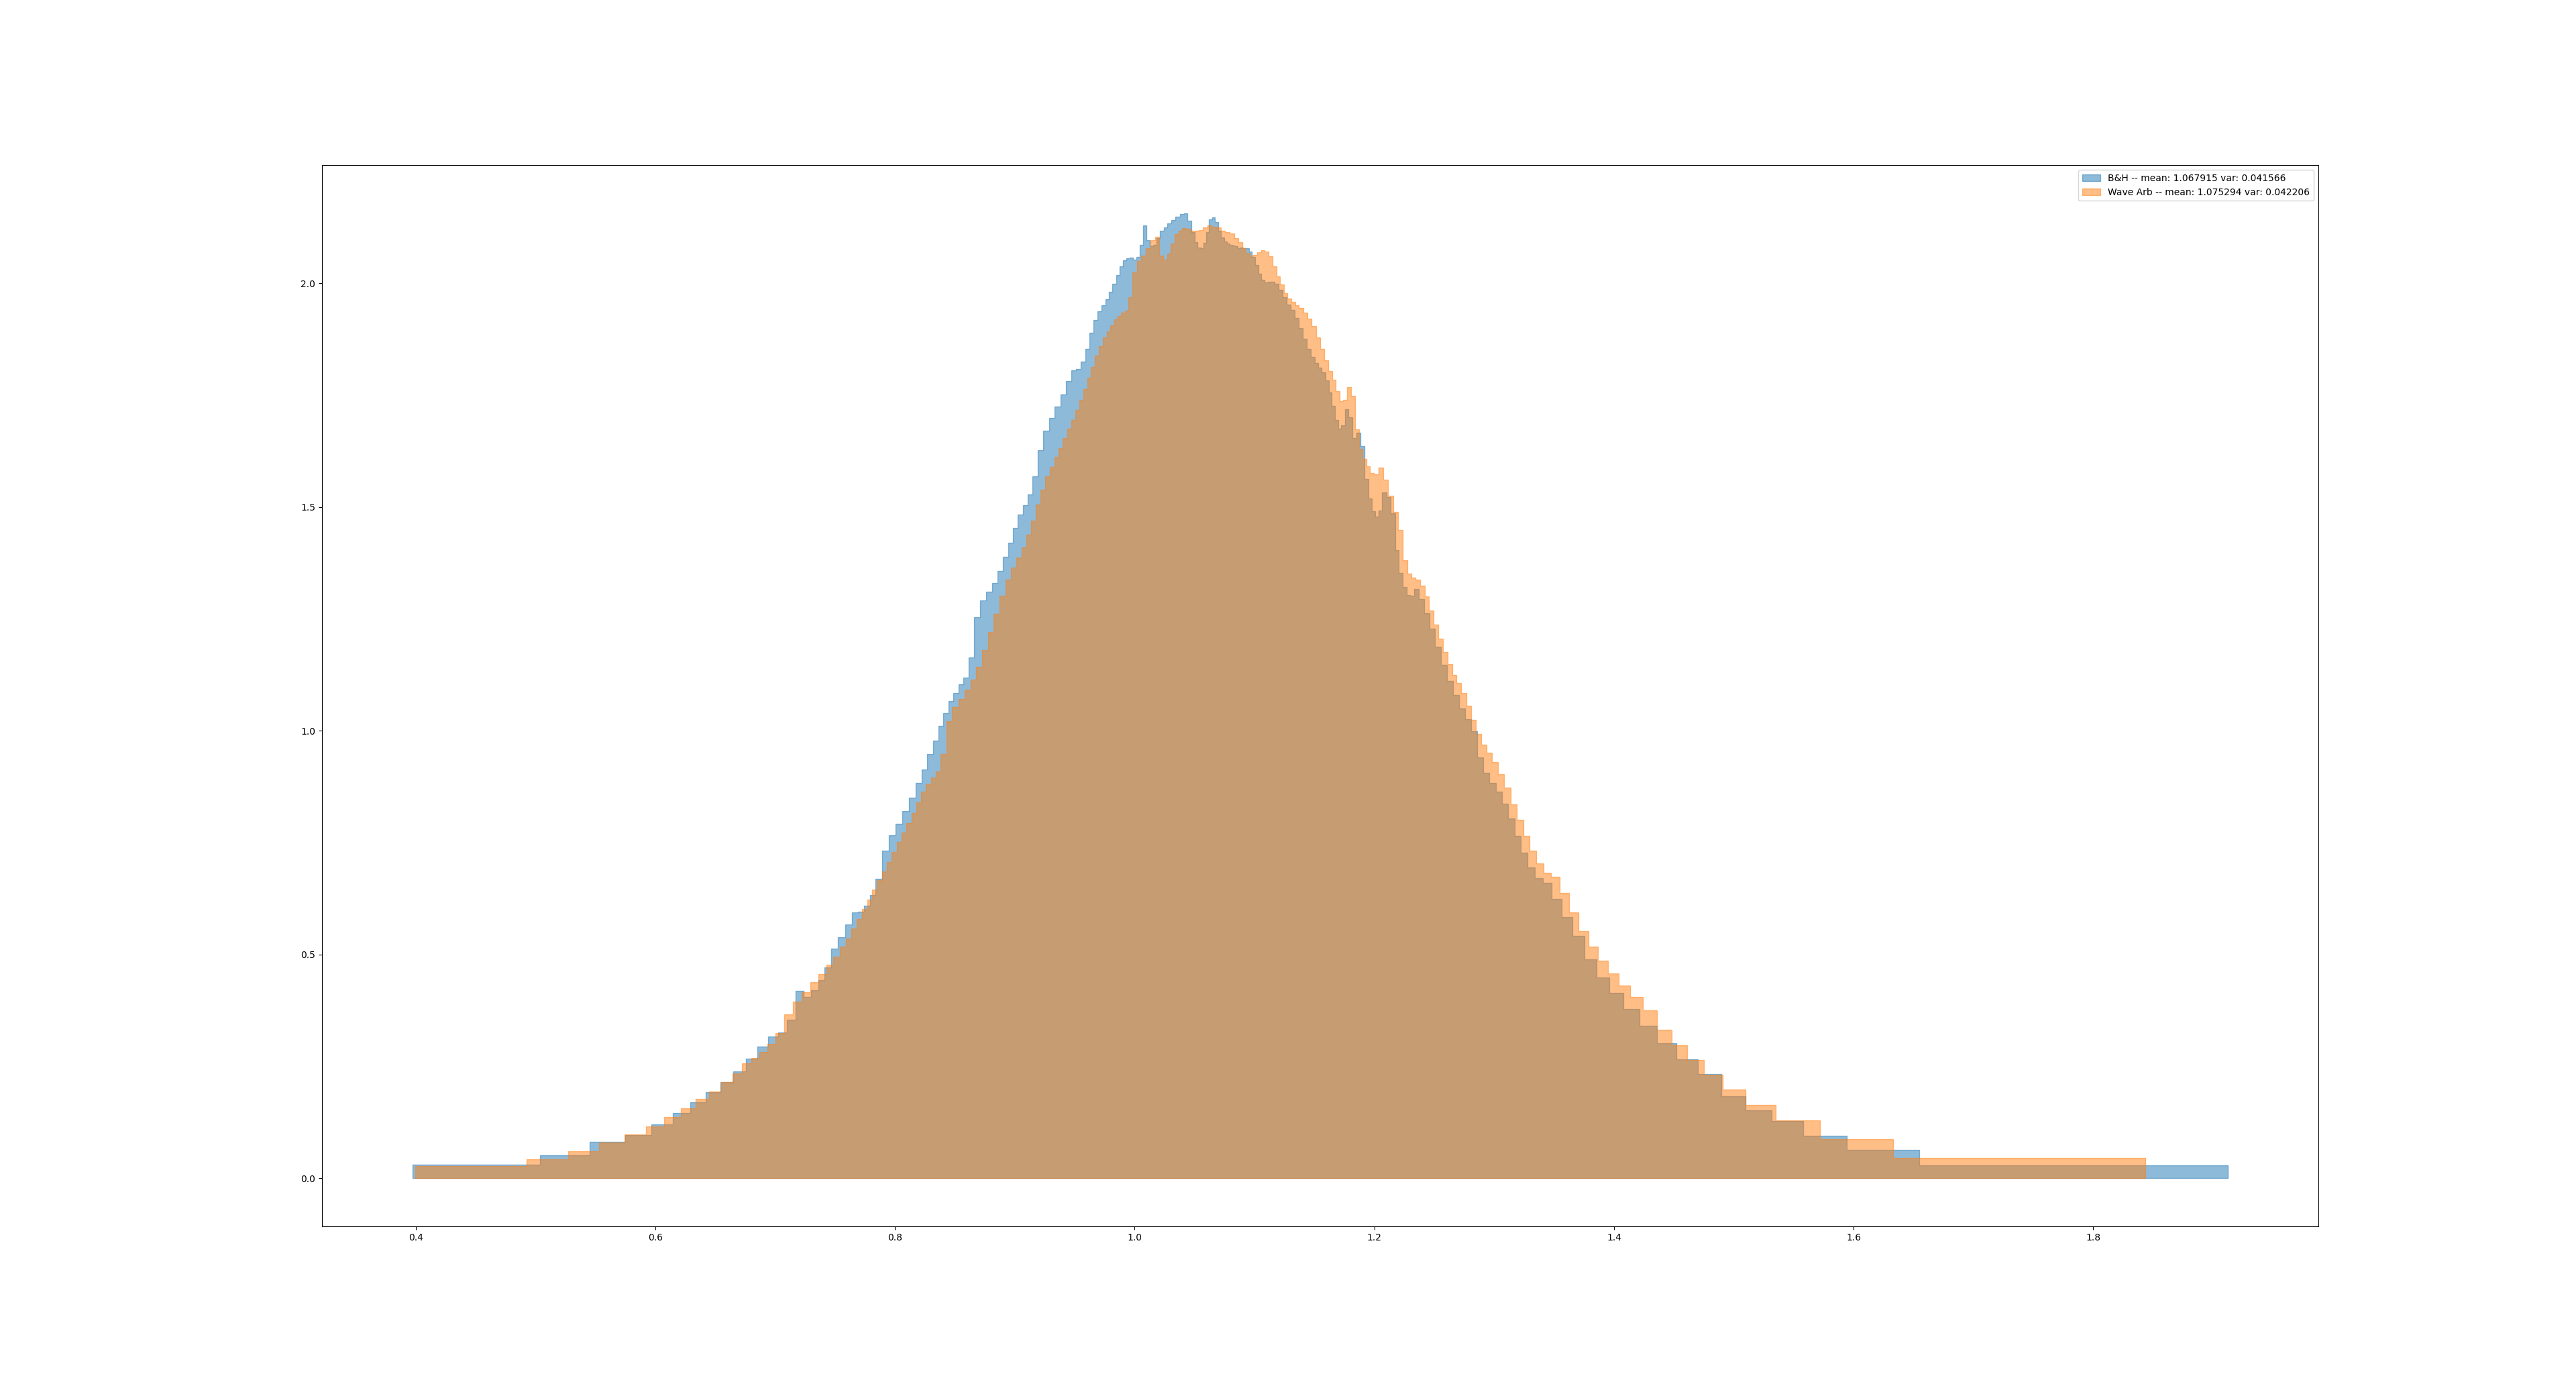
\includegraphics[width=\linewidth]{OneYearReturnRates.png}
  \caption{One Year Return Rates}
  \label{fig}
\end{figure}

This simulation uses 438 stocks listed on the SP500. It avoids any SP500 stock
that had a split or reverse split, as well as any stock that stopped trading
during the four year span. Dividends are reinvested.

This simulation does not make any attempts to avoid slippage effects, so we
encourage researchers with more sophisticated back test frameworks to verify
these results.

Each pair of assets was modeled and over 26 billion data points for one year
returns were collected into the histograms in Figure \ref{fig}. The final
result is that wave arbitrage outperformed the buy-and-hold strategy by an
average of $0.75\%$.

\section{Conclusions}

In order to reach the conclusions in Section \ref{sec:disproof}, we made the following assumptions:

\begin{itemize}
  \item Price movements are a ``fair game'' and follow a martingale.
  \item Prices fluctuate with respect to each other.
  \item Prices do not go to zero.
  \item The efficient market hypothesis can be stated in terms of expected
        returns.
\end{itemize}

When prices follow a sub martingale, the disproof of Section \ref{sec:disproof}
no longer works. Simulations for the sub martingale generated by using a fair coin and taking

\begin{equation}
  p_{t+1} =
    \begin{cases}
      k p_t         & \mbox{if heads,} \\
      \frac{p_t}{k} & \mbox{if tails,}
    \end{cases}
\end{equation}

suggest that the expected values for wave arbitrage and the buy-and-hold are
equal. However, the variance of results for wave arbitrage is substantially
lower than those of buy-and-hold.

The assumption that prices do not go to zero is debatable since companies go
bankrupt every year. When the prices for an asset do go to zero, the value of a
portfolio managed by wave arbitrage also go to zero. Additional rules should be
developed to deal with this scenario. It is not clear whether the assumption
that prices do not go to zero poses any serious challenge to the disproof in
Section \ref{sec:disproof}.

It is unclear what might happen if a substantial portion of a market is
governed by wave arbitrage. Perhaps markets would become less volatile.
However, since the efficient market hypothesis is false, it is also possible
that other algorithms would be able to take advantage of the wave arbitrage
algorithm.

\bibliographystyle{unsrtnat}
\bibliography{references}

\end{document}
